\documentclass[10pt,letterpaper,twocolumn]{article}

\usepackage[T1]{fontenc}
\usepackage{lmodern}
\usepackage[margin=0.62in,columnsep=0.27in]{geometry}
\usepackage{amsmath,amssymb,mathtools}
\usepackage{array,booktabs}
\usepackage{graphicx}
\usepackage{xcolor}
\usepackage{microtype}
\usepackage{fancyhdr}
\usepackage{needspace}

\graphicspath{{figures/}}

% The user-local tools/array package is newer than the available LaTeX kernel.
\makeatletter
\def\vcenter@text{\vbox}
\makeatother

\definecolor{navy}{HTML}{17365D}
\definecolor{green}{HTML}{2F6B4F}

\pagestyle{fancy}
\fancyhf{}
\fancyhead[L]{\footnotesize Holstein-dimer stability addendum}
\fancyhead[R]{\footnotesize Offline closure diagnostic}
\fancyfoot[C]{\thepage}
\renewcommand{\headrulewidth}{0.3pt}

\setlength{\parindent}{0pt}
\setlength{\parskip}{2.7pt plus 0.4pt}
\renewcommand{\arraystretch}{1.08}

\newcommand{\R}{\mathbb R}
\newcommand{\ii}{\mathrm i}
\newcommand{\segmenthead}[1]{%
  \Needspace{4\baselineskip}%
  \par\smallskip{\color{navy}\large\bfseries #1}\par
  \vspace{-2pt}{\color{navy}\rule{\columnwidth}{0.7pt}}\par\smallskip
}
\newcommand{\conceptbreak}{%
  \par\smallskip\noindent
  {\color{black!30}\rule{\columnwidth}{0.35pt}}%
  \par\smallskip
}

\begin{document}
\raggedbottom
\setcounter{page}{24}

\twocolumn[
\begin{center}
  {\color{navy}\Large\bfseries Replacement Pages 24--25}\par\vspace{2pt}
  {\large Offline Reconstruction of the Missing Correlation Velocity}\par\vspace{2pt}
  {\small Continuation after the previously printed page 23, 2 August 2026}
\end{center}
\vspace{2pt}\hrule\vspace{5pt}
]

\segmenthead{The two derivatives being compared}

The retained correlation is the pair
\[
C=(C^0,C^1),
\qquad C^q\in\mathbb C^{2\times2},
\]
with one electron--phonon correlation matrix for each phonon mode
\(q\in\{0,1\}\).  The symbol \(\dot C_{31}\) is the derivative assigned to
this pair by the uncorrected 31-real-coordinate archive closure.  It is the
\(C\)-block of the closure velocity \(f(t,x)\):
\[
x\xrightarrow{\mathcal E}X=(\rho,B,N,A,C)
\xrightarrow{F_C}\dot C_{31}.
\tag{X44a}
\]
Printed Eq. (D14d) evaluates that block as
\[
\boxed{
\dot C_{31}^{,q}
=-\ii\bigl(h(t)C^q-C^qh(t)+\omega_qC^q\bigr)
+\sum_{a=0}^{4}S_a^q.}
\tag{X44b}
\]
The commutator and \(\omega_qC^q\) transport the existing correlation.  The
five archive sources \(S_a^q\), displayed in printed Eq. (D3), create and
modify it using only the retained matrices \(\rho,N,A\).

The exact reference begins from the same initial state and driven truncated
Holstein Hamiltonian.  Adaptive DOP853 propagates the full wavefunction
\(\lvert\psi_{\rm ex}(t)\rangle\).  At each saved time, contraction gives
\(X_{\rm ex}(t)\), and the Hamiltonian commutator gives the exact retained
derivative:
\[
\lvert\psi_{\rm ex}(t)\rangle
\longrightarrow X_{\rm ex}(t),
\qquad
\dot X_{\rm ex}(t)=\ii\langle[H,\widehat X]\rangle_t.
\tag{X44c}
\]
The archive equation is then evaluated on that same exact contracted state:
\[
\dot C_{31}(t)
=F_C\bigl(t,X_{\rm ex}(t)\bigr),
\qquad
\dot C_{\rm ex}(t)
=\ii\langle[H,\widehat C]\rangle_t.
\tag{X44d}
\]
This common input isolates a local equation error: the difference comes from
the derivative formula, rather than from two trajectories having already
separated.

\conceptbreak
\textbf{Why the archive derivative is incomplete.}
Let
\[
O_{ij}=c_{j\uparrow}^{\dagger}c_{i\uparrow},
\qquad
n_{r\uparrow}=c_{r\uparrow}^{\dagger}c_{r\uparrow},
\qquad
\delta X_r=\delta b_r+\delta b_r^{\dagger}.
\]
The exact equation requests the mixed expectation
\[
Q^{qr}_{ij}
=\left\langle
[O_{ij},n_{r\uparrow}]\delta X_r\delta b_q
\right\rangle.
\tag{X44e}
\]
The second-order closure replaces it by the product
\[
Q^{qr}_{ij,0}
=\left\langle[O_{ij},n_{r\uparrow}]\right\rangle
 \left\langle\delta X_r\delta b_q\right\rangle.
\tag{X44f}
\]
Their connected remainder
\[
K^{qr}_{ij}=Q^{qr}_{ij}-Q^{qr}_{ij,0}
\tag{X44g}
\]
records the correlation between the electronic commutator fluctuation and the
phonon-pair fluctuation that the product closure removes.

Two electronic covariances enter at the same operator line:
{\footnotesize
\[
\begin{aligned}
P^q_{ij}
&=\operatorname{Cov}(O_{ij},n_{q\uparrow})
=\delta_{iq}\rho_{qj}-\rho_{ij}\rho_{qq},\\
D^q_{ij}
&=\operatorname{Cov}(O_{ij},n_{q\downarrow})\\
&=\langle O_{ij}n_{q\downarrow}\rangle
-\rho_{ij}\langle n_{q\downarrow}\rangle.
\end{aligned}
\tag{X44h}
\]
}
The fixed-number identity determines \(P\) from \(\rho\); \(D\) carries
opposite-spin information absent from the 31 retained coordinates.

\segmenthead{The three supplied velocity terms}

The connected mixed-moment contribution is
\[
\boxed{
\Delta\dot C^q_{K,ij}
=-\ii g\sum_{r=0}^{1}K^{qr}_{ij}.}
\tag{X44i}
\]
For the Pauli term, the archive sources already contain an effective
same-spin contribution.  The repair subtracts that archive contribution and
supplies the exact covariance:
{\footnotesize
\[
\boxed{
\Delta\dot C^q_{P,ij}
=-\ii gP^q_{ij}
-\left[
\left(\sum_{a=0}^{4}S_a^q\right)_{ij}
+\ii g\sum_rQ^{qr}_{ij,0}
\right].}
\tag{X44j}
\]
}
The opposite-spin contribution is
\[
\boxed{
\Delta\dot C^q_{D,ij}=-\ii gD^q_{ij}.}
\tag{X44k}
\]
Consequently the exact local derivative decomposes as
\[
\boxed{
\dot C_{\rm ex}
=\dot C_{31}
+\Delta\dot C_K
+\Delta\dot C_P
+\Delta\dot C_D
+R_{\rm cut}.}
\tag{X44l}
\]
The final term is the finite-cutoff commutator remainder,
\[
R_{\rm cut}
=\dot C_{\rm ex}-\dot C_{31}
-\Delta\dot C_K-\Delta\dot C_P-\Delta\dot C_D.
\tag{X44m}
\]

\conceptbreak
\textbf{How the offline attribution was performed.}
Let \(\mathcal R_C\) extract the fourteen independent real coordinates of
\(C=(C^0,C^1)\).  For a supplied set
\(S\subseteq\{K,P,D\}\), define
{\scriptsize
\[
\begin{aligned}
e_S(t)=\mathcal R_C\Bigl(&
 \dot C_{31}(t)+\sum_{\alpha\in S}\Delta\dot C_\alpha(t)
 -\dot C_{\rm ex}(t)\\
&-\dot C_{31}(0)-\sum_{\alpha\in S}\Delta\dot C_\alpha(0)
 +\dot C_{\rm ex}(0)\Bigr).
\end{aligned}
\tag{X44n}
\]
}
The second line removes the constant \(t=0\) residual.  The remaining curve
measures how well each supplied source follows the driven change of the exact
correlation velocity.

Sequential substitution over \(0\leq t\leq4\) gives
\[
\begin{array}{@{}lrr@{}}
\toprule
S&\operatorname{RMS}\lVert e_S\rVert_2
&\max_t\lVert e_S\rVert_2\\
\midrule
\varnothing&0.166690&0.274310\\
K&0.089345&0.137864\\
K+P&0.026160&0.038268\\
K+P+D&2.53\times10^{-5}&3.47\times10^{-5}\\
\bottomrule
\end{array}
\tag{X44o}
\]

\begin{center}
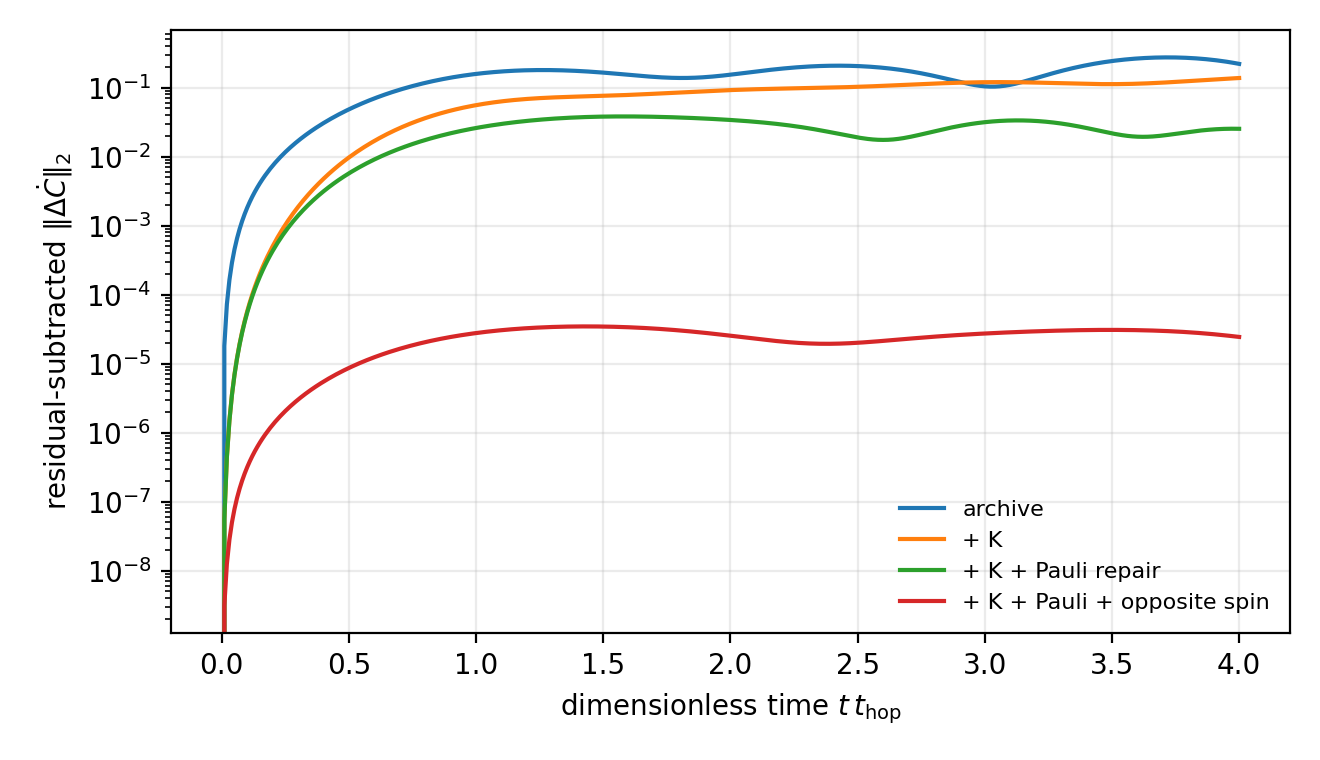
\includegraphics[width=\columnwidth]{exact_mixed_moment_closure_attribution.png}

\parbox{0.96\columnwidth}{\scriptsize
\textbf{Sequential reconstruction of the missing \(C\)-velocity.}
Every curve evaluates the archive derivative on the exact cutoff-16 trajectory.
Orange supplies \(K\), green then supplies \(P\), and red finally supplies
\(D\).  The red curve reaches the finite-cutoff remainder scale.}
\end{center}

\newpage
\conceptbreak
\textbf{What this establishes.}
The successive decrease demonstrates that \(K\), the Pauli repair \(P\), and
the opposite-spin covariance \(D\) account for the evolving local
\(C\)-derivative defect to the finite-cutoff floor.  It measures derivative
accuracy at exact-trajectory samples.  It does not report the accuracy of a
newly propagated \(K+P+D\) trajectory.

The calculation was offline.  Exact wavefunctions supplied \(K\), \(P\), and
\(D\) only for source attribution.  These terms were never inserted into RK4
and were never inputs to the representability controller.  The
minimum-Euclidean-norm controller \(w\) enforces the matrix physicality,
trace, and energy conditions on the approximate velocity.  The
\(K,P,D\) audit identifies the missing dynamics that a future autonomous
closure must generate from its own enlarged state.

\end{document}
